\cleartooddpage[\thispagestyle{empty}]
\chapter{VERITAS}\label{chapter:veritas}

\begin{figure}[ht]
  \begin{center}
    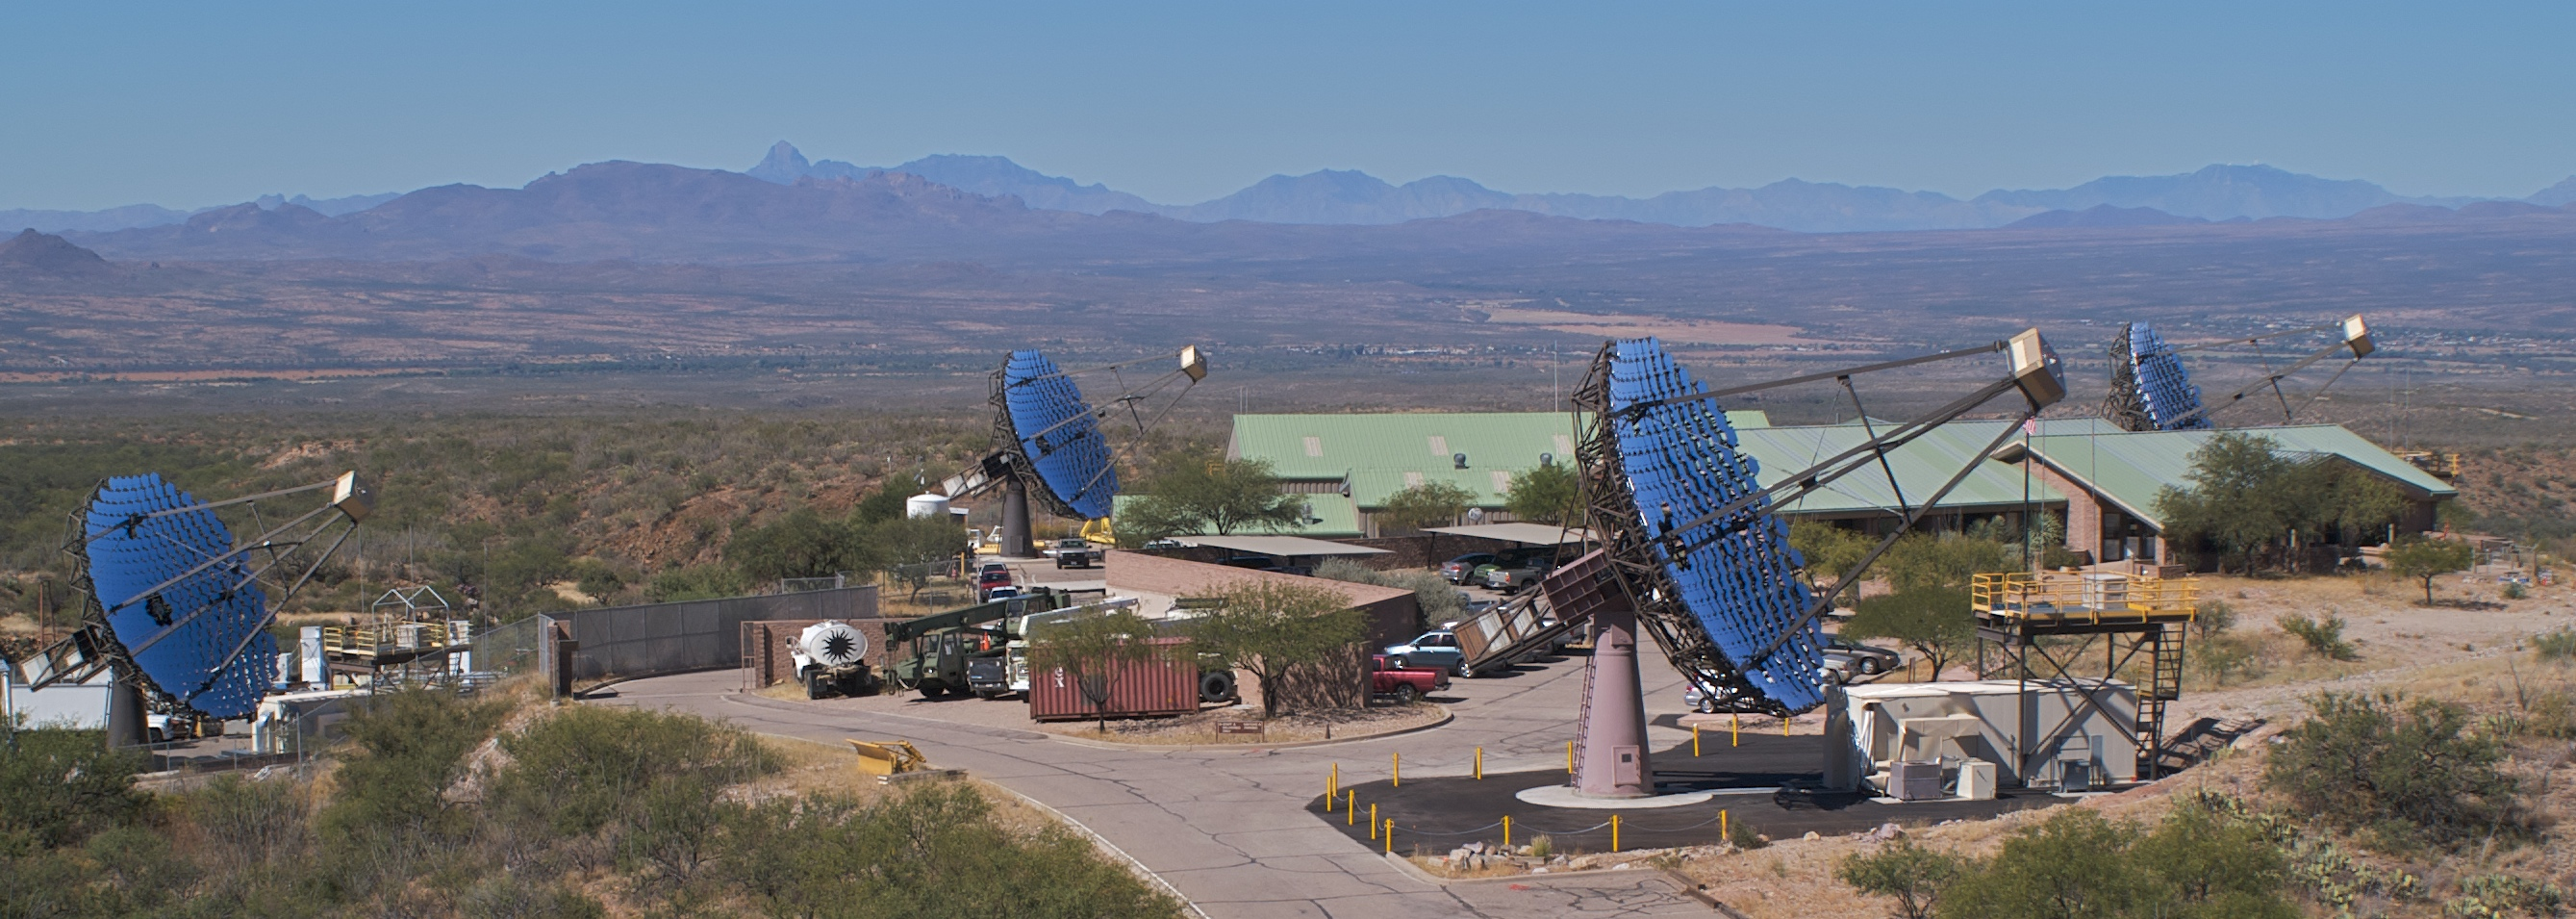
\includegraphics[width=0.95\textwidth]{images/veritas_array_v6}
    \caption[VERITAS Array]{The VERITAS observatory.}\label{fig:veritasarray}
  \end{center}
\end{figure}

VERITAS (Very Energetic Radiation Imaging Telescope Array System, pictured in figure \ref{fig:veritasarray}) is a gamma ray observatory operating in Arizona, USA, and is capable of detecting $\nicetilde$TeV-energy gamma rays.
The observatory consists of an array of four Imaging Atmospheric Cherenkov Telescopes (IACTs), each spaced $\nicetilde$90m apart.
Each telescope possesses an array of 345 mirrors, and a Photomultiplier Tube (PMT) camera (containing 499 PMTs) on a set of struts.
When a gamma ray produces an air shower in the atmosphere, the shower emits blue-UV Cherenkov photons over a timespan of nanoseconds.
By focusing these photons onto the PMT camera with the mirrors, images of the shower can be taken, where each pixel of the image consists of analog voltage pulses from each PMT, with more photons causing larger pulses.


%As the width of voltage pulses must be \nicetilde{}ns to prevent overlapping with the pulses from other showers, the digization hardware measures the time-dependent voltage of each pulse in 1-nanosecond-wide(??) time bins.
%Though faint showers may only posess a few photons per PMT, brighter showers can still shine several thousand photons onto individual pixels.
%This means that the digization hardware must be able to handle a large dynamic range of inputs, over several orders of magnitude in voltage.
%To accomplish this, two amplification levels are used in the digization circuit, High Gain for voltage pulses of a few photons, and Low Gain for voltage pulses of several thousand photons.

In the following sections, the different hardware components are examined, in order of signal propagation.
In section \ref{sec:telpoint}, the Telescope Pointing is discussed, including its monitoring and calibration.
The Mirrors are discussed in section \ref{sec:mirrors}, including their properties and alignment.
In section \ref{sec:pmts}, the PMTs are discussed, including their performance and calibration.
The trigger system is discussed in section \ref{sec:trig}, relating how candidate signal voltages are saved while discarding those sourced from noise.
In section \ref{sec:epochs}, the different observatory epochs are discussed, as over time changes and modifications have changed the observatory's performance.


\section{Telescope Pointing}\label{sec:telpoint}

\begin{figure}[ht]
  \begin{center}
    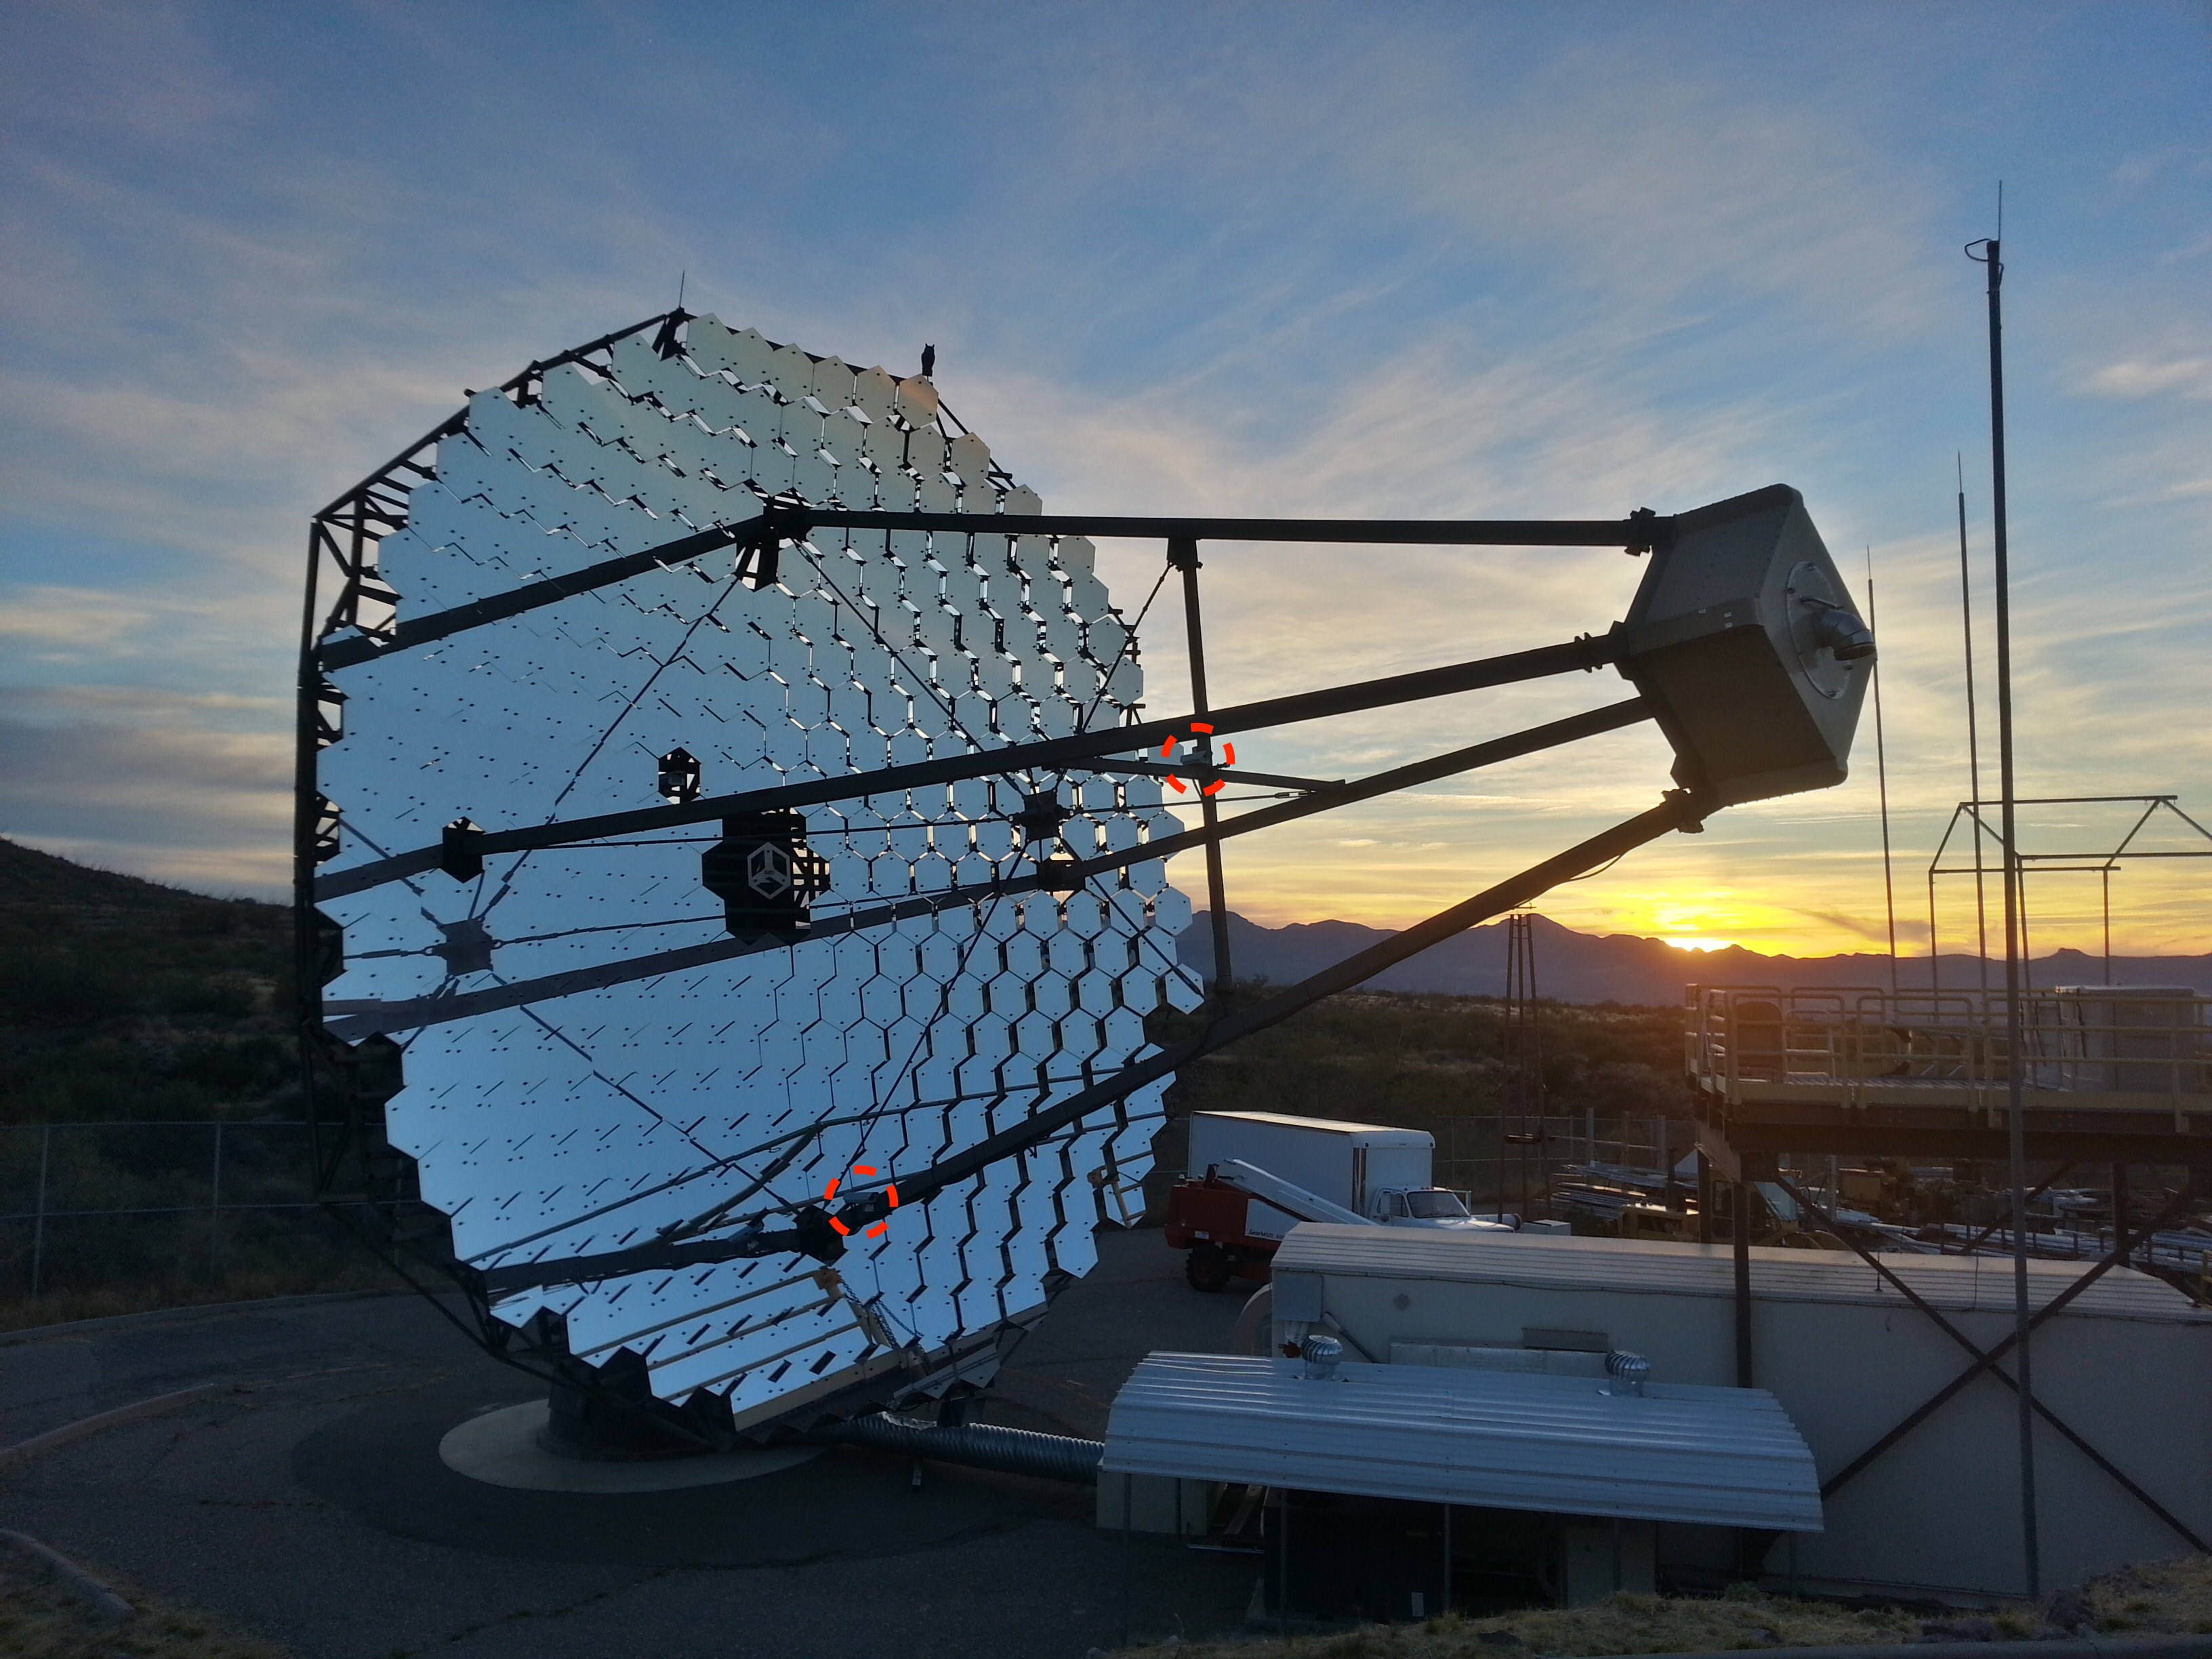
\includegraphics[width=0.95\textwidth]{images/single_telescope}
    \caption[Single Veritas Telescope]{View of the 345 mirrors, the support structure, and the PMT Camera housing at the end of the four supporting arms.}\label{fig:davcottel}
  \end{center}
\end{figure}

Like most telescopes, each VERITAS telescope has an immobile base, and a pointable dish for collecting light.
This dish can rotate in azimuth and in elevation, with enough range in both axes to point at any direction above the horizon.
At their fastest, the telescopes can slew at a rate of $ \nicetilde \ang{1} $ per second.
To track where the telescopes are pointing, the motors that drive the azimuth and elevation movement have encoders that digitize the pointing direction of the dishes.
However, as the dishes are large metal structures, they bend and flex at different elevations and azimuths.
To account for this flexing, the encoder values are then given to a structural model called T-Point, which corrects for the dish structure bending at different azimuths and elevations.
After applying this model, the telescope pointing can be tracked with an accuracy of $\ang{0.013}$ to $\ang{0.027}$ (That is a range within a factor of two. Why?? -Gernot) \cite{Veritas_Detector}.

As an improvement to the encoder measurements, a VERITAS Pointing Monitor (VPM) system is also in place.
The VPM consists of two CCD cameras fixed to each telescope, pointing parallel to the telescope pointing, and a set of LED lights attached to the PMT camera, next to the Winston cones (see section \ref{sec:pmts}).
The first CCD camera is attached below the bottom mirrors, and images the stars in the field of view.
The second CCD camera is attached to the support struts, roughly halfway between the mirrors and the camera, and images the focal plane of the telescope.
Both cameras are marked by red dashed-line circles in figure \ref{fig:davcottel}.
During regular observations, these cameras take images of background stars and the focal plane LEDs every two seconds and matching the star positions, an improved pointing accuracy of $ \ang{0.0069} $ (And you are sure it ..69, and not ....70?? -Gernot) can be achieved.
%originally in griffin thesis 2016, pg45, but is there a better citation??

As the VERITAS telescopes are based on old designs for a military solar concentrator that sets targets on fire \cite{daviescotton}, the VERITAS telescopes have similar abilities.
This mostly means that care must be taken during the day to point the telescopes away from the sun during maintanance and storage.
% 100m^2 * 1000w/m^2 = 100,000W
If any direct sunlight falls onto the telscope mirrors, the \nicetilde100,000 Watts of light will be concentrated either onto the camera, or a point within a few meters of the camera, which could potentially cause signficant damage to telescope hardware or nearby plants, animals, and people.
VERITAS telescopes are stored during the day by pointing them North at $ \nicetilde \ang{0} $ elevation.

( Missing here is the relevance for your thesis. Does the VPM work with the same accuracy at 30 deg? What about the encoders? What is the minimum elevation possible?? -Gernot)

\section{Mirrors}\label{sec:mirrors}

When the Cherenkov light from a gamma-ray shower first interacts with the telescope array, it is by being reflected by some of the 345 mirrors.
These mirrors face towards the incoming Cherenkov light, with the PMT camera facing the mirrors, as shown in figure \ref{fig:davcottel}.
When its spherical mirrors, spherical dish, and focal length ratio of $ \nicetilde 2 $ are considered, this configuration is referred to as a Davies-Cotton telescope \cite{daviescotton}.
Each mirror has an area of 0.322$m^2$, and a spherical curvature radius of 24m.
The mirrors are each mounted along the support structure so that the total diameter of the telescope's mirror area is 12m, with a total area of 111$m^2$ and a focal length of 12m \cite{Veritas_Detector}.
The mirrors' reflectivity as a function of wavelength is shown in figure \ref{fig:mirreflect}.
The VERITAS specifications state that the mirror reflectivity must be $\geq 85\%$ between 280nm and 450nm.

\begin{figure}[ht]
  \begin{center}
    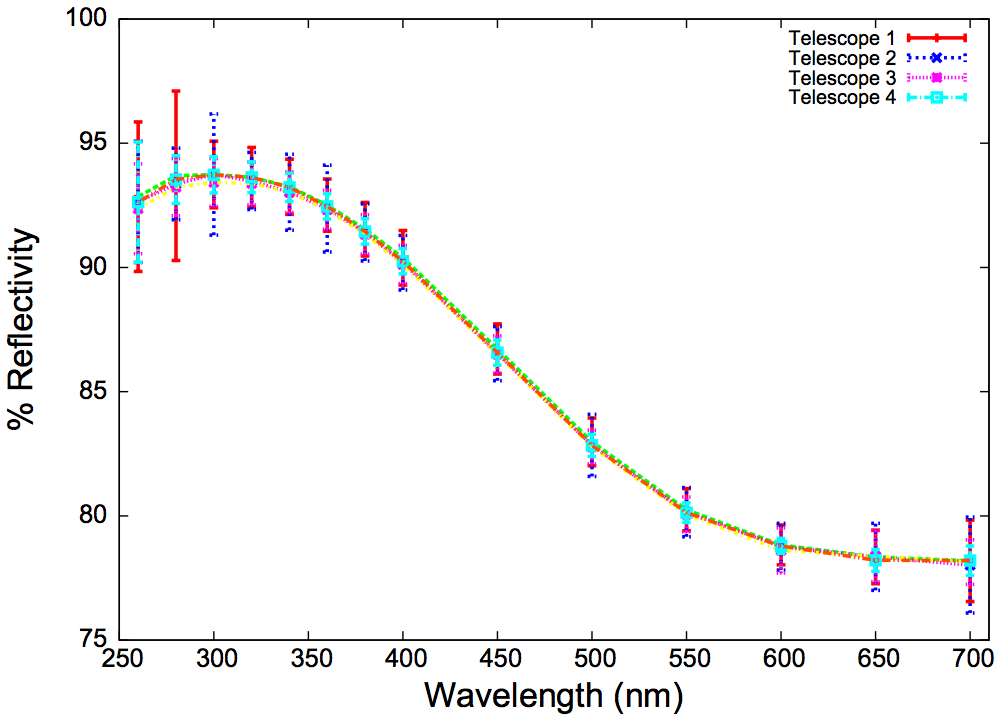
\includegraphics[width=0.75\textwidth]{images/mirror_reflect}
    \caption[Mirror Reflectivity]{Mirror reflectivity as a function of wavelength for each telescope, from Ref \cite{mirrorfacets}. (Really?? All points are exactly on top of each other -Gernot)}\label{fig:mirreflect}
  \end{center}
\end{figure}

As the mirrors are exposed to the elements, they slowly accumulate dust and scratches.
To combat this, they are cleaned and recoated every two years.
Each mirror is attached to the support structure via three adjustable mounting points, allowing for adjustment of the mirror orientation to point directly at the camera, as detailed in \cite{mirroralign}.
This alignment is measured and adjusted at regular intervals, using background stars as a calibration source.

(Why is the PSF so important for your thesis?? -Gernot)


\subsection{Star Point Spread Function}

Due to dust, minor imperfections in the surface of the mirrors, and small mirror misalignments, the photons that bounce off the mirrors are not reflected perfectly.
Instead, a single point-like light source appears smeared out on the focal plane.
This smearing is then quantified by a fitted gaussian function, usually called the optical Point Spread Function\footnote{Please note that this is different from the PSF described in Chapter \ref{ch:grrecon}, which quantifies the spread in the reconstructed gamma-ray positions.  The optical PSF instead describes the spread of UV-Optical photons.} (PSF).
By pointing a telescope at different stars and placing a CCD at the focal plane, the mirror PSF is measured monthly.
The first VERITAS telescope's first calibration image shown in figure \ref{fig:mirrorpolaris}.
The mirror psf roughly gaussian-shaped but with longer tails, with a $ \ang{0.06} $ full width half maximum \cite{Veritas_Detector}.

\begin{figure}[ht]
  \begin{center}
    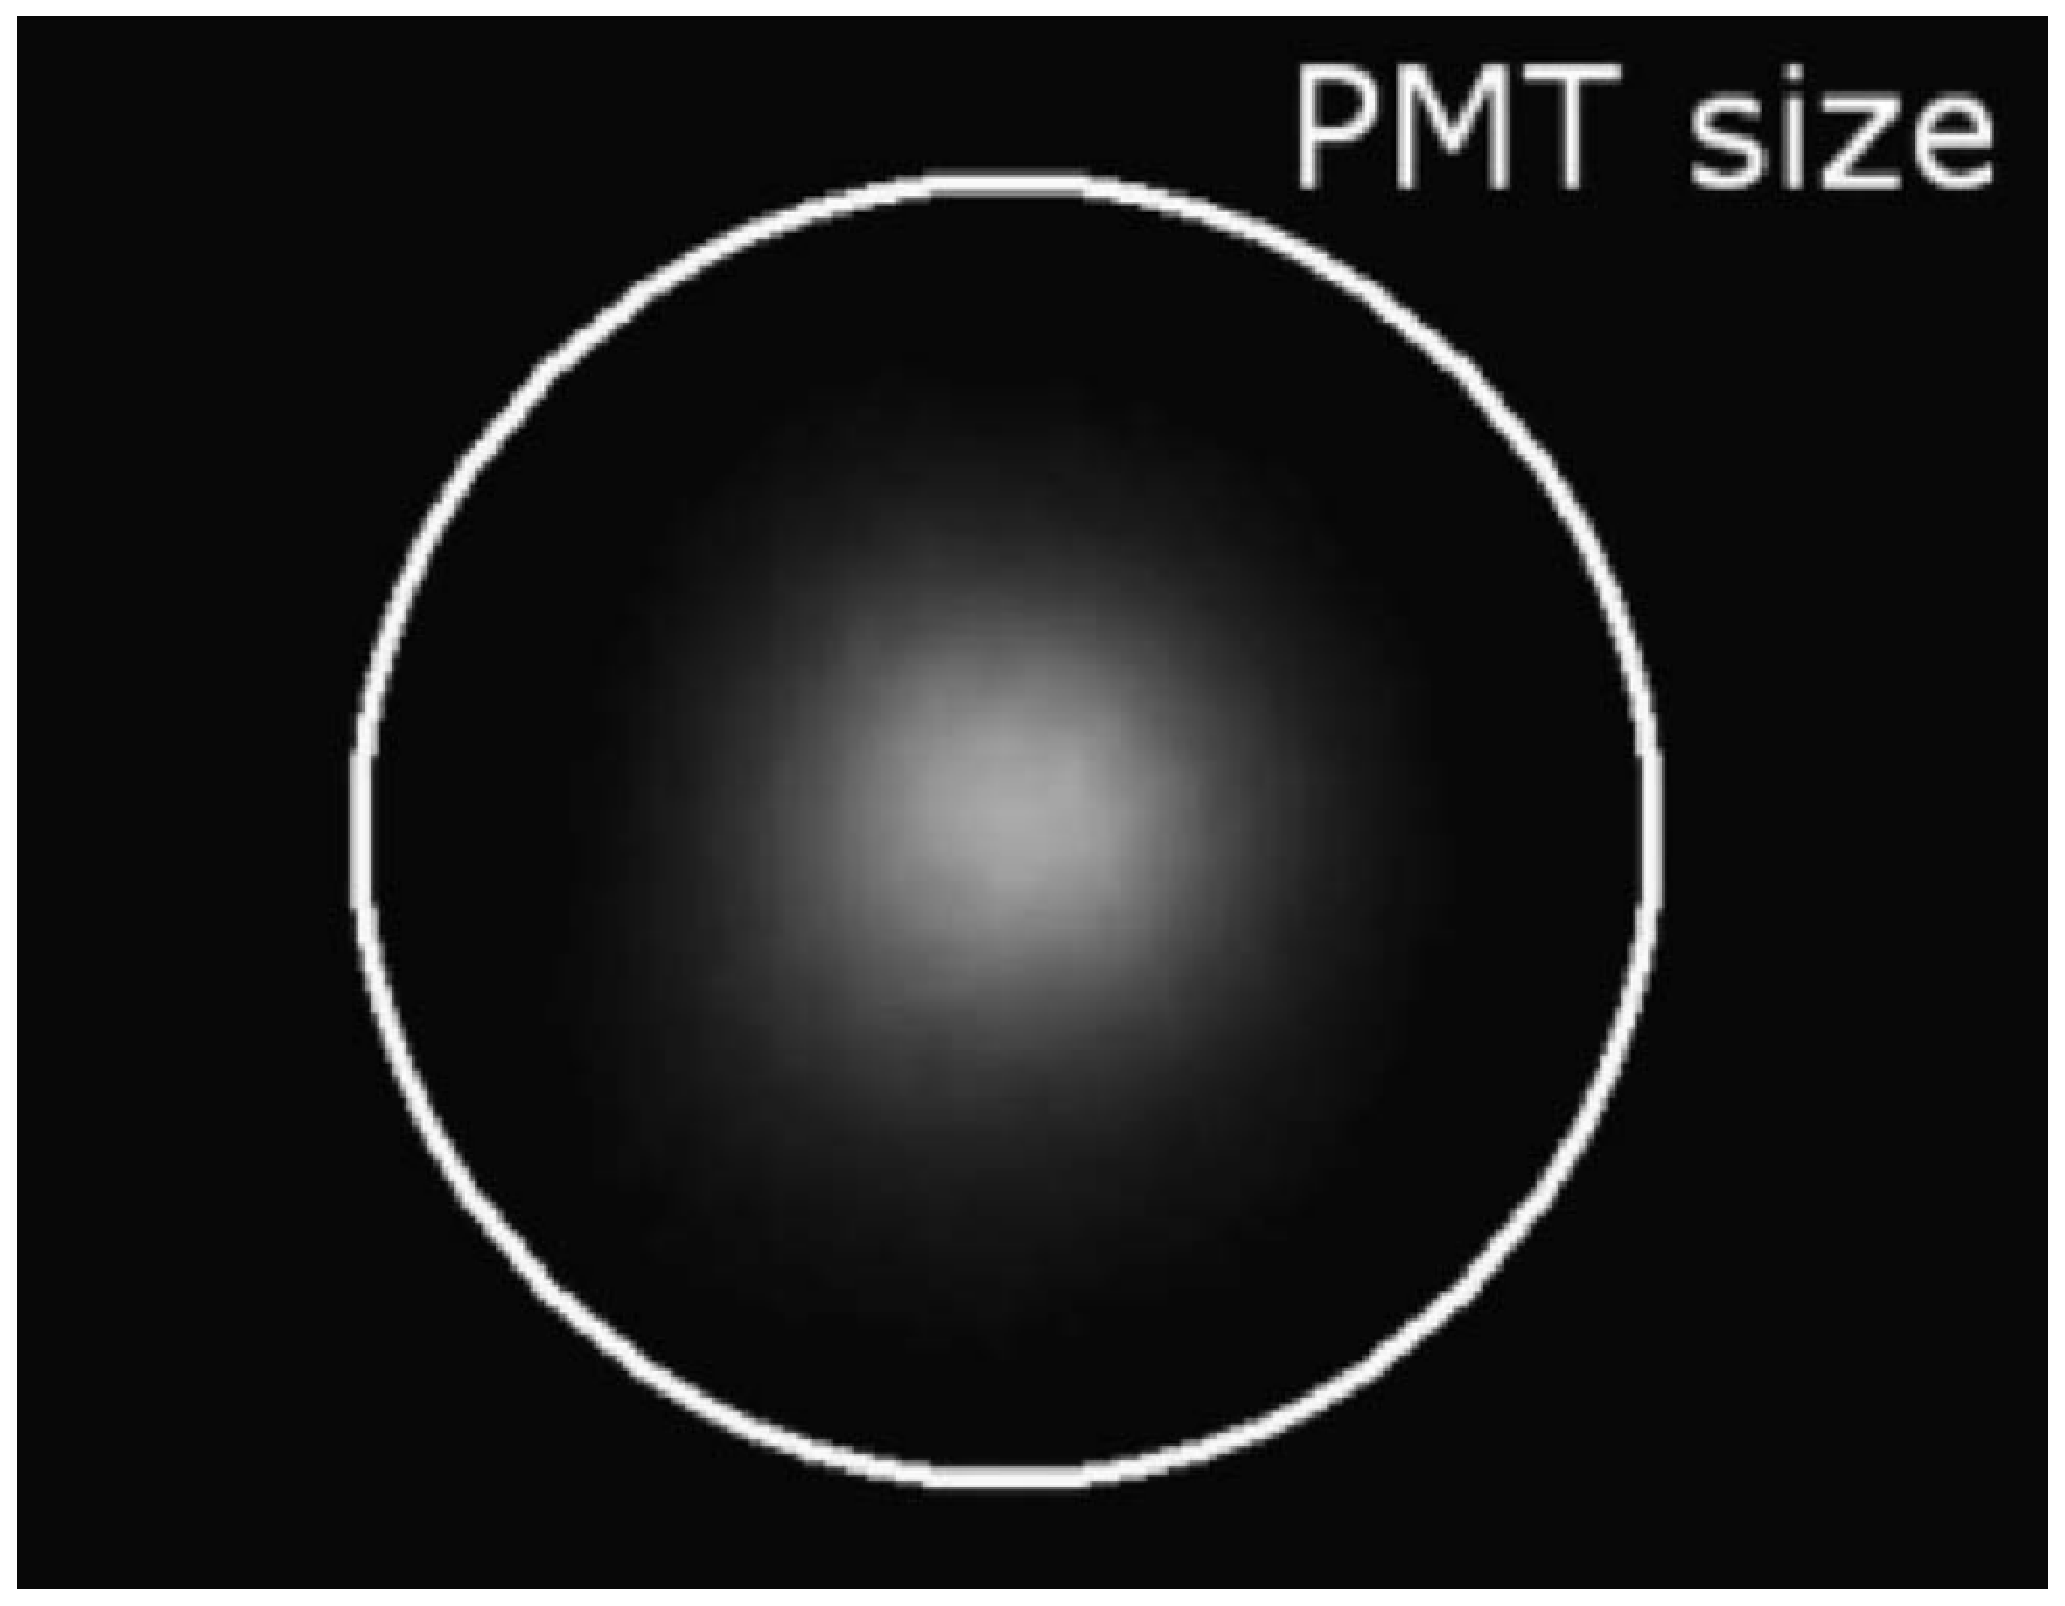
\includegraphics[width=0.75\textwidth]{images/mirror_polaris.eps}
    \caption[Polaris PSF]{Image of Polaris after reflecting off the mirrors, demonstrating the mirror Point Spread Function, from \cite{Veritas_Detector}.  The circle indicates the radius of a PMT.}\label{fig:mirrorpolaris}
  \end{center}
\end{figure}

\subsection{Mirror Alignment}
% https://veritas.sao.arizona.edu/wiki/index.php/Mirror_Alignment
The mirror alignment procedure is performed by placing a CCD camera at the focal plane, facing towards the mirrors.
The telescope is then pointed towards a magnitude 2 star at $ \nicetilde \ang{70} $ elevation.
The pointing is known as a `raster' scan of the star, where each mirror's field of view is in turn centered on the star.
By using the CCD to examine the position of the star in each mirror, the mirror's alignment can be calculated and corrected.



\section{PMTs}\label{sec:pmts}

Each telescope has a PMT Camera on the end of four supporting arms, inside a protective housing.
This camera consists of 499 Photo Multiplier Tubes (PMTs), each with a Winston cone to increase the light collection area for each PMT.
The PMTs are Hamamatsu's model R10560-100-20 MOD \cite{pmtmodels}.
These winston cones can be seen attached to the PMTs in figure \ref{fig:winstcones}.

\begin{figure}[ht]
  \begin{center}
    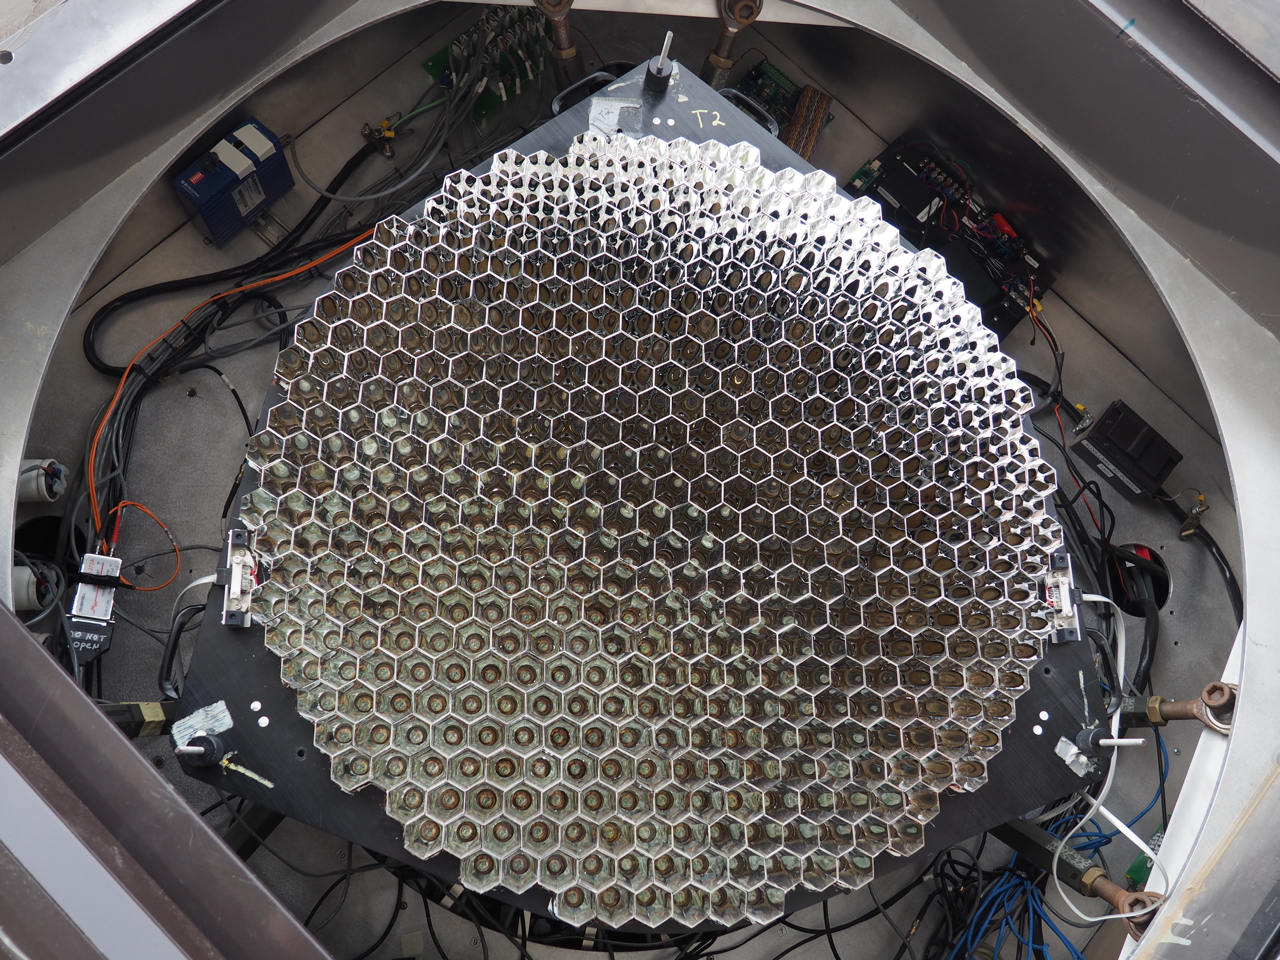
\includegraphics[width=0.75\textwidth]{images/winston_cones_t2}
    \caption[Winston Cones]{Hexagonal Winston cones over the circular PMTs, inside the camera housing.}\label{fig:winstcones}
  \end{center}
\end{figure}


\begin{figure}[ht]
  \begin{center}
    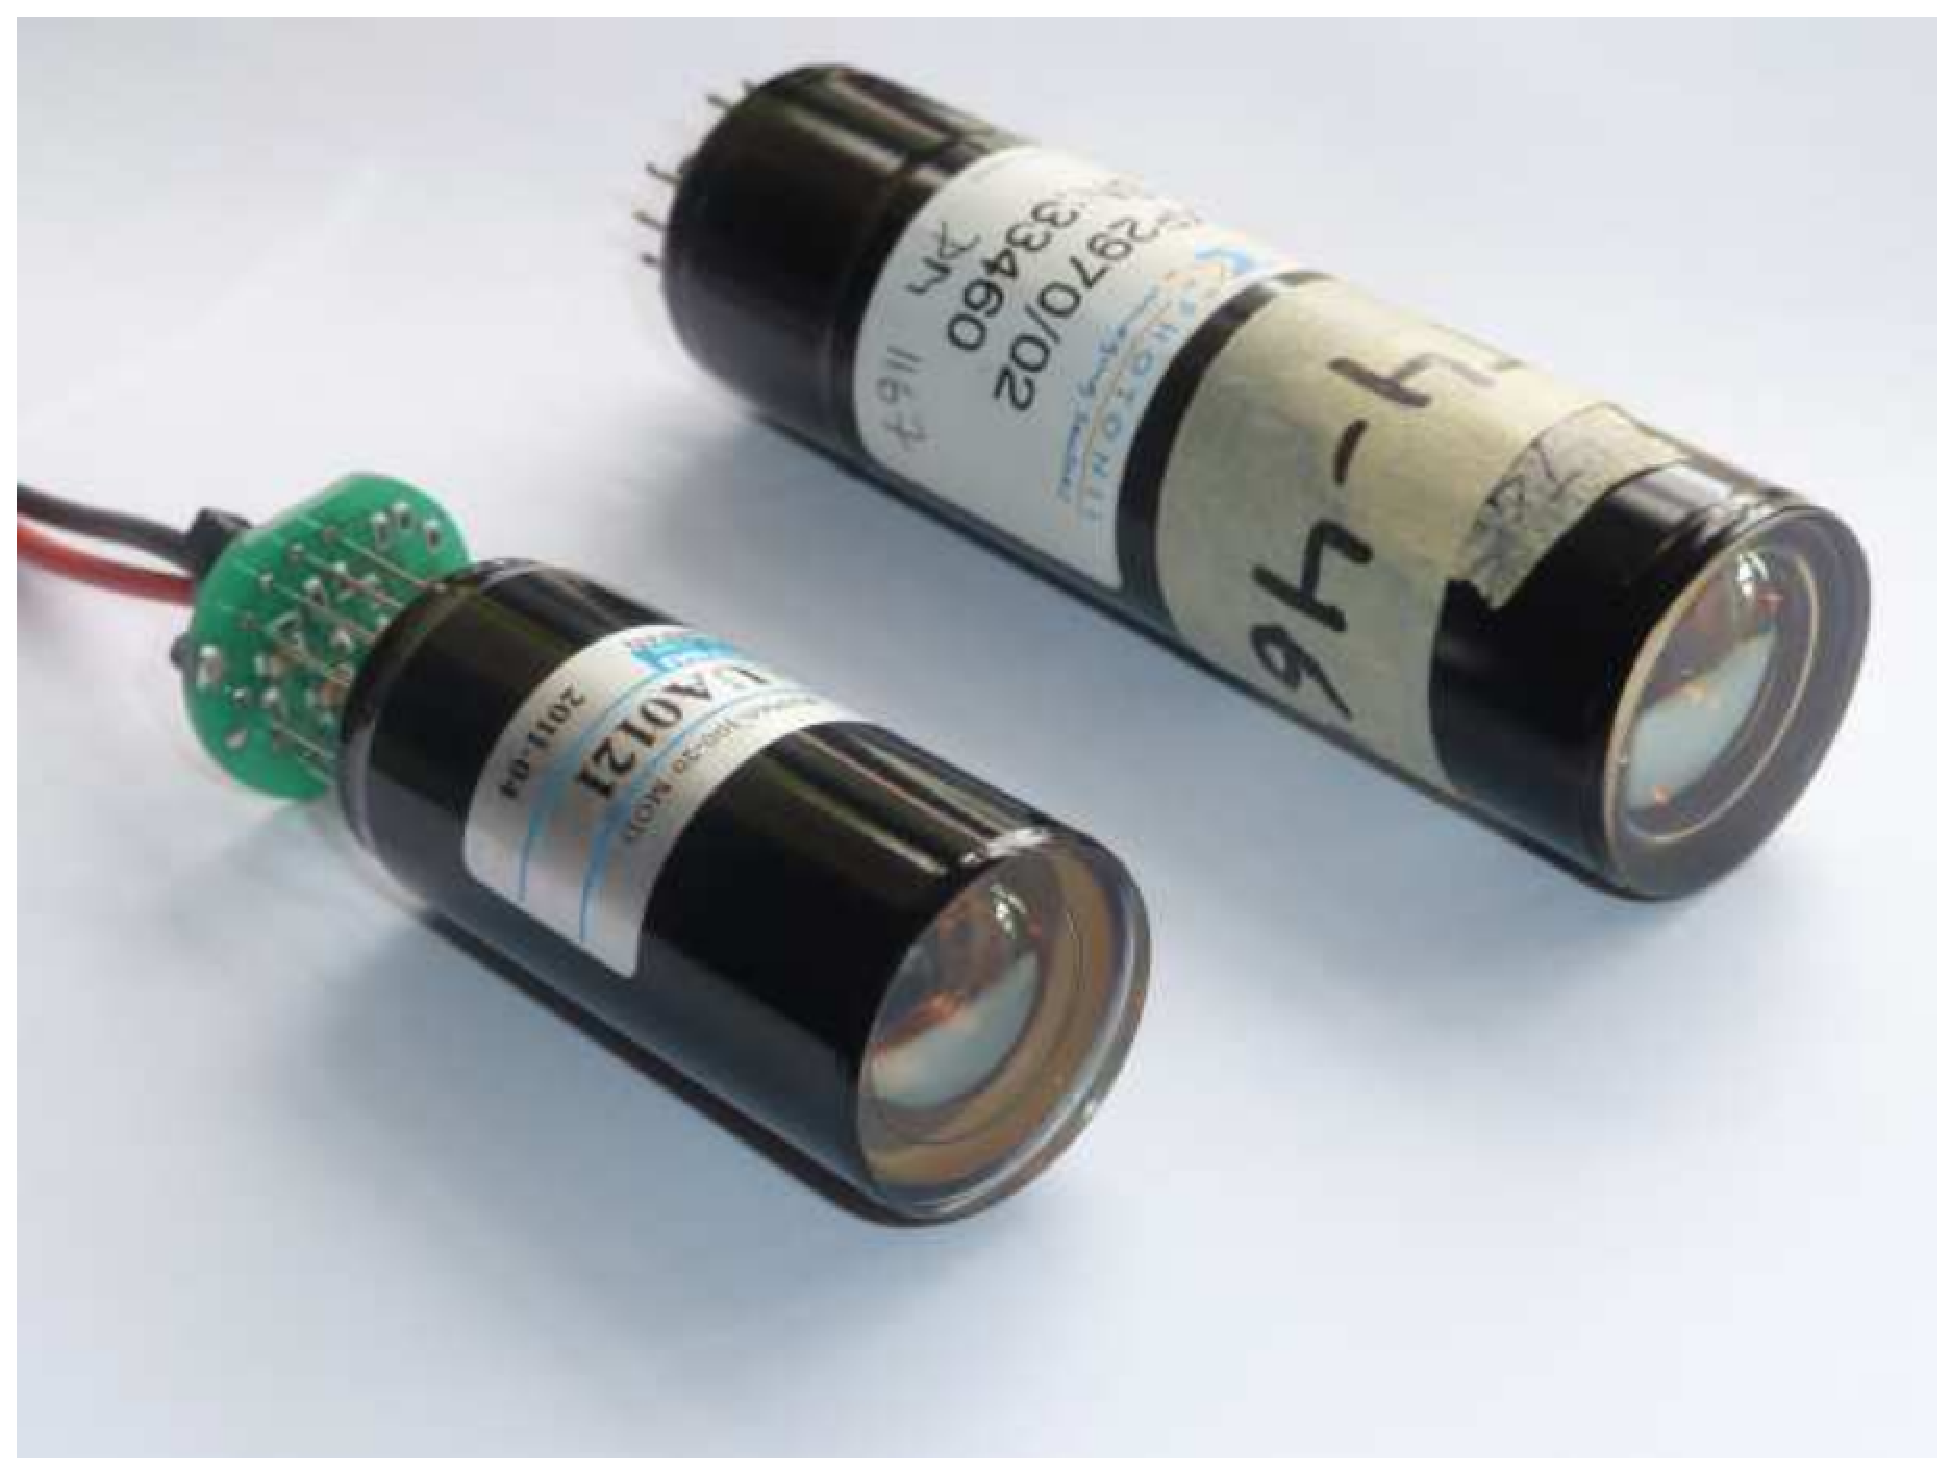
\includegraphics[width=0.75\textwidth]{images/pmt_models}
    \caption[PMT Models]{The two PMT models used in the VERITAS cameras. \cite{pmtmodels}}\label{fig:pmtmodels}
  \end{center}
\end{figure}

To operate, the PMTs are connected to high voltage, typically around several hundred Volts.
(?? Be exact here, you know the voltage much better -Gernot)
The PMTs' output signals are first sent through an amplifier, before travelling down a \nicetilde45m cable to trigger and digitization electronics stationed near the telescope, which digitize the signal.

The first circuit that the signal passes through is a Constant Fraction Descriminator (CFD) circuit.
This circuit duplicates the signal voltage pulse from the PMTs, inverts and delays the duplicate pulse, and adds it back to the original pulse.
This combined pulse then crosses the zero-volts threshold (called a Zero Threshold Descriminator) at the same time (how 'same'?? within 1 ns??) as the original pulse reaches its peak, acting as a maximum-voltage detection circuit.
When a maximum voltage is detected by the circuit, it emits a 10ns trigger pulse to other electronics.

(add diagram of CFD pulses??)

The use of this circuit has two main benefits.
The first use is that the CFD circuit will trigger at the same time regardless of the pulse size (??).
If a simple threshold trigger is used to detect a signal pulse, the time of the trigger will be earlier for larger pulses, and later for smaller pulses.
The CFD's zero threshold trigger is invoked when the signal voltage pulse is at 75\% of its maximum value. (cite??)

The second use is that when the CFD circuit detects a voltage pulse larger than a given maximum threshold, it can emit an extra logic trigger, called a low-gain trigger.
This extra low-gain trigger is then used by the FADC to switch between high-gain and low-gain mode when digitizing voltage pulses.

%CFD behavior cite??

%CFD model??

%FADC model??

After the CFD emits a trigger pulse, the signal voltage pulse is passed to another circuit for digization, a Flash Analog-to-Digital Circuit (FADC).
This FADC circuit then, for each nanosecond time bin, measures how large the voltage pulse is with a series of 255 (??) constant-voltage thresholds.
The highest threshold that is crossed in a single time bin then determines the digital voltage value that is saved to the FADC buffer for that time bin.

(?? Please read the T1 paper again, this paragraph is not entirely correct -Gernot)
If the low-gain trigger pulse was also recieved by the FADC, then the signal voltage pulse is de-amplified(means attenuated, or reverse the effect of the previous amplification??) before being digitized, since the CFD low-gain threshold is set to lower than the FADC maximum digitizable voltage.
If this low-gain triggering did not take place, then the FADC would become saturated.
Once the voltage pulse is digitized, it is saved to a rolling buffer (how long is the buffer??) in the FADC, waiting for higher level triggers, signaling the FADC to readout its buffers into a datafile.

\subsection{PMT Upgrade}
In summer of 2012, all PMTs in the telescopes were replaced with improved PMTs.
Specifically, the original Photonis XP2970 models were replaced with the Hamamatsu R10560-100-20 MOD.
This was done because that R10560 has a considerably higher quantum efficiency (\nicetilde$90\%$ (??this is not the right value??)), compared to the XP2970 (\nicetilde$75\%$(??this is not the right value??)).
This higher quantum efficiency means more photons from a shower are detected by the PMT, which means VERITAS is more sensitive to lower energy gamma rays \cite{pmtmodels}.
In addition, the voltage pulse due to a single photoelectron is shorter with the R10560 compared to the XP2970, as shown in figure \ref{fig:pmt_pulse_widths}.

\begin{figure}[ht]
  \begin{center}
    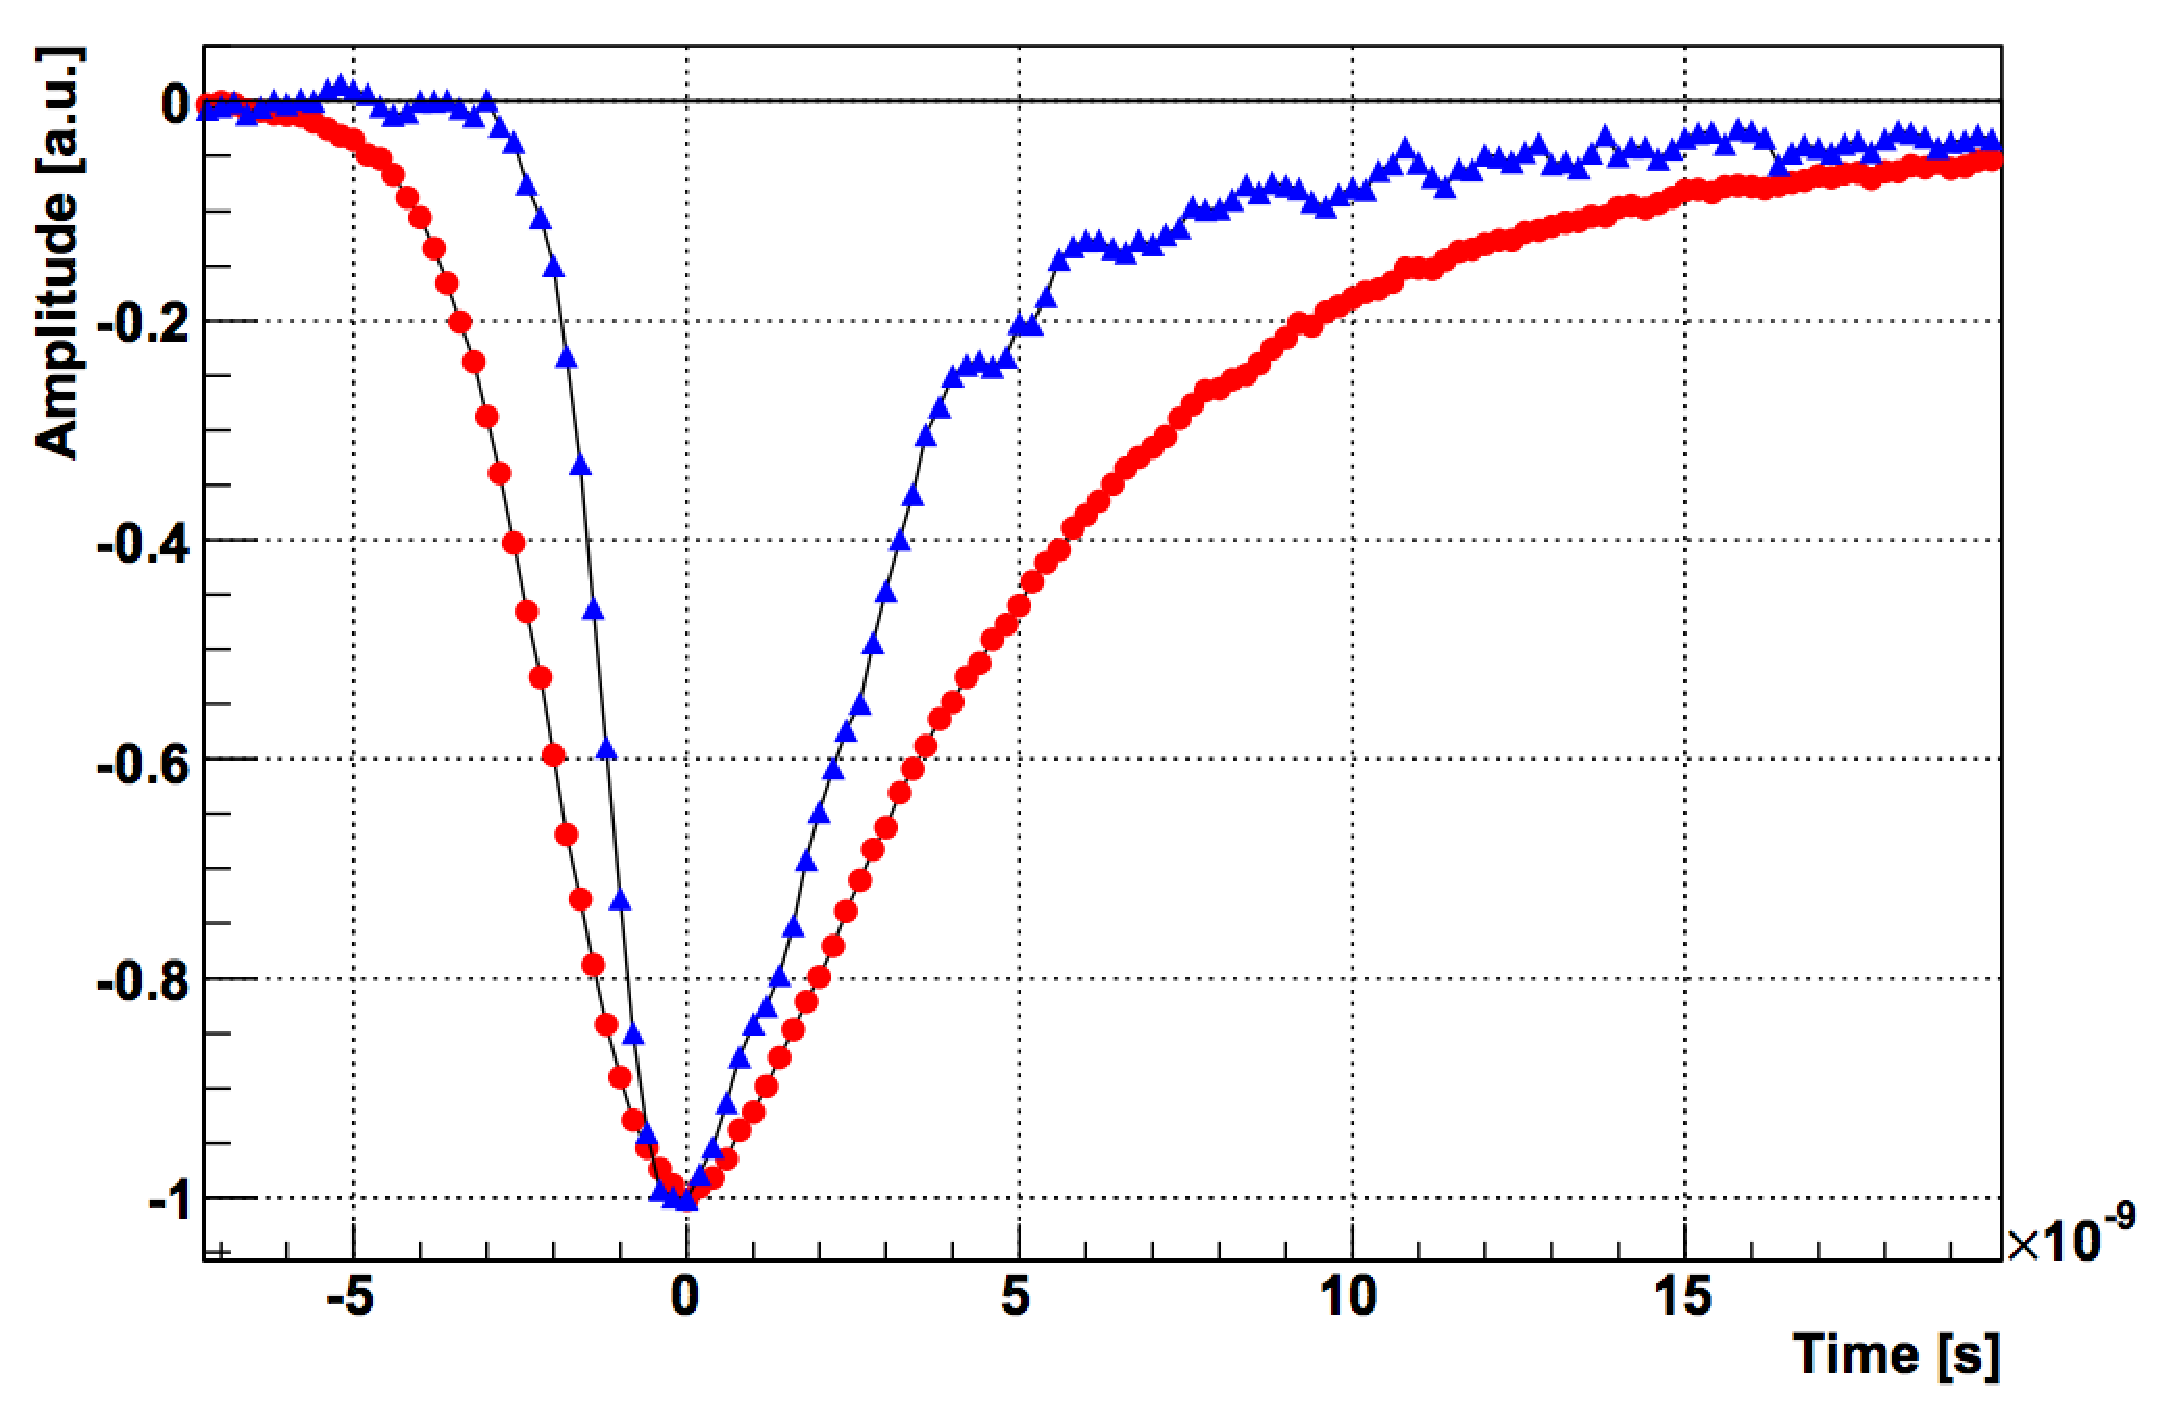
\includegraphics[width=0.75\textwidth]{images/pmt_models_pulsewidths.eps}
    \caption[Pulse Shapes]{Pulse shapes of the old XP2970 PMTs (red circles) and the new R10560 PMTs (blue triangles), taken from \cite{pmtmodels}.  Plots are the average of many afterpulses, normalized to the maximum amplitude.  Pulses shown include dispersion due to a \nicetilde55m coaxial cable between the PMTs and the digitizer boards.}\label{fig:pmt_pulse_widths}
  \end{center}
\end{figure}

(if I don't use V4/V5 data at all, I should discuss them less (??))
The data used in this thesis was taken after the upgrade, which means the telescope performance is different for these two time periods.
This is accounted for by separate simulations for each PMT model, mostly resulting in different effective areas at the lower energies.


\subsection{PMT Calibration}

While the VERITAS PMTs are all the same model, there are still differences from PMT to PMT that can impact any data taken.
Primarily, these differences can cause the same number of incident photons to create differently-shaped output voltage pulses in each PMT.
To account for these differences, there are several calibration procedures that are applied nightly or semi-nightly.
These are performed with a set of flashing LEDs, placed next to the mirrors such that they illuminate the PMTs.

((??) No. that paragraph is completely wrong. We never look at the pulse width. We do not adjust the HV nightly -Gernot)
In the first procedure, the LEDs are flashed at \nicetilde10Hz (100 or 300?? -Gernot) at the beginning of each night.
While the LEDs are flashing, the average pulse width from each PMT is monitored.
Then, the High Voltage is adjusted for each group of PMTs to make their pulse widths as similar as possible (there are several PMTs connected to each high voltage crate).
This must be done nightly, because just like each PMT is unique, each PMT's temperature dependence is also unique.

In the second procedure, once every several nights the single-photoelectron curves for each PMT are measured.
This is done by placing an opaque (several-mm-thick metal) plate over the PMTs, with a single 3.1mm (diameter?? radius??) hole drilled over the location of each PMT.
The LEDs are then flashed repeatedly.
As the opaque plate has holes for each PMT, each PMT gets on average 0-5 photons per flash.
Large numbers of flashes can then be used to gather information on each PMTs' distribution of pulse widths.
By examining a histogram of the pulses' integrated charges, one can see poisson-statistics peaks that are formed for the 1, 2, 3, and further integer numbers of photons.
These peaks can then be used to translate the digital counts from the PMTs into their originating photoelectrons.
These calibration techniques are further detailed in \cite{calib_techniques}.

(Figure describing poissonian peaks??)



\section{Trigger System}\label{sec:trig}

The operation of VERITAS requires digitizing voltage pulses with voltage samples roughly once per nanosecond, per photomultiplier tube.
This means that, with 255(??) voltage levels, 1 second of raw voltage data would require 2 Terabytes of space.
As this is unfeasable with today's computing systems, only subsets of the raw pixel voltages are saved when certain trigger conditions are met.
To complicate matters, photons from atmospheric muons and the night sky background can also cause voltage pulses similar to a gamma ray shower's cherenkov photons.
Thus, VERITAS has a system of triggers that reduces the amount of raw data that is saved, while also partially filtering out non-gamma-ray events.

The L1 is the first and lowest level trigger.
An L1 trigger (sometimes called a pixel trigger) is emitted when a PMT's CFD circuit detects a signal voltage above a given threshold, typically in the 10s of mV.
This threshold voltage is varied throughout datataking by a rate-feedback system, which adjusts the trigger threshold according to the night sky background level.

((??) Again, this paragraph is far too detailed and not relevant -Gernot)
The L2 (image) trigger is emitted by the FPGA when a group of L1 triggers meet certain requirements.
These requirements include that multiple L1 triggers must fall within a certain time window, and that multiple L1 triggers form one of several predefined shapes, or templates.
The coincident time window varies. (elaborate??)
There are several patterns. (elaborate??)
The pattern requirements help reduce the number of triggers from non-gamma-ray sources.
Night sky background photons are only able to trigger individual pixels, and muons tend to create ring-shaped images.
Once one of these patterns occurs within a time window, the FPGA emits an L2 trigger, which is sent to the L3 (array) trigger system.

The L3 (array) trigger system, is a computer, which looks for coincident L2 triggers that fall within a \nicetilde50ns time window.
This window is varied for each telescope based on the azimuth and elevation of the pointing, as these can introduce delays between images of up to 100s of nanoseconds.
During a typical observation period, the L3 trigger rate is around 200-300Hz.

Once an L3 trigger is invoked, a signal is sent to all telescopes that the digitized voltages for all pixels in the cameras should be read out from their buffers, and saved to memory.
These pixel voltages are then processed by the analysis software to reconstruct the gamma-ray events.



\subsection{Deadtime}
When the L3 trigger is invoked and the buffers are being read out, the FADCs are unable to store new PMT voltages in the buffers.
Being unable to store new PMT voltages effectivly reduces the amount of time spent observing gamma rays.
This lost time is usually referred to as deadtime.
As the deadtime is a fixed time loss per event, the percent of time lost due to event readout rises with the a higher frequency of readouts.
This means that at an L3 trigger rate of \nicetilde300Hz, approximately \nicetilde12\% of the time is lost due to buffer readouts.
Since the L3 rate varies over the course of a single 30 minute run, this means that the deadtime also varies.
This is accounted for in the flux calculation in section ??.

\subsection{Time Zero Calibration}
As all PMTs and signal cables are not identical, there are differences in how long a voltage pulse takes to travel.
More specifically, the time between a) when the photon strikes the PMT's photocathode and b) when the voltage pulse sets off its L1 trigger, can vary from pixel to pixel.
This is usually measured by looking at the average arrival time of many events over all camera pixels.
By looking at the average arrival time, pixels that are consistanly early or late can be accounted for, which improves image identification.

\section{Epochs}\label{sec:epochs}
After being built, VERITAS has evolved over several years, with collaboration members upgrading it to improve performance.
However, these major differences need to be taken into account in the analysis chain.
To organize these differences, in the data they are referred to as epochs 1, 2, 3, 4, 5, and 6 (usually denoted as V1, V2, V3, V4, V5, and V6).
For telescope positions, the following coordinate system in meters is used.
For the telescope positions, a coordinate system is used where the origin of is at 31.675N, 110.962W, the x axis points East, and the y axis points North.

As the first three telescopes were constructed and brought online, data taken after each was brought online are considered the first, second, and third epochs.
Telescope 1 was placed at (-37.6, -23.7), telescope 2 at (44.1, -47.7), and telescope 3 at (29.4, 60.1).
In 2007, the fourth telescope was constructed at (-35.9, 11.3), and data taken between this point in time and the next major upgrade is considered the fourth epoch (V4).

In September 2009, telescope 1 was moved to a new position (135.4, -8.61), after it was demonstrated with simulations that it would grant a \nicetilde30\% improvement in sensitivity \cite{veritas_t1_move}.
Data taken after this relocation is referred to as the fifth epoch (V5).

In August 2012, the PMTs in all cameras were replaced with improved PMTs that had a higher quantum efficiency, improving the telescopes ability to resolve images \cite{pmtmodels}.
Data taken after this upgrade is considered part of the sixth epoch (V6).

As these different epochs have different telescope configurations, the instrument response functions are different, meaning each epoch behaves in a quantifiably distinct manner.
For the Dark Matter analysis described in this thesis, only data from the sixth epoch is used.


